\chapter{Majorization Pressed Harder}\label{chap:mmcollatz}

\Cref{chap:lyapunov} showed that the linear majorizer\index{majorization} of $\log x$ cannot certify descent.
This chapter asks what the majorization idea can do for
the Collatz map when it is pushed as far as it will go. We obtain four things.
First, the natural majorizer of a Syracuse stride is multiplicative, not
linear; summed around a cycle, its bound \emph{is} the cycle
inequality on which \cref{chap:cycles} builds, and its minorizer is the window lemma\index{window lemma} of that chapter. The
cycle half of the conjecture becomes the question of how tight this majorizer
can be made along a closed orbit, a reformulation rather than a method. Second, a potential that corrects $\log x$ by a bounded
function of residues is impossible, and the reason is a negative cycle
condition from shortest path theory: the residue graph of the map contains,
for every modulus, cycles of positive mean weight, among them the images of the cycles of $T$ on
the negative integers\index{negative cycles}. Third, any pointwise potential must assign a surplus to
integers with a run of trailing ones that grows linearly in the length of the
run. Fourth, majorizing over a whole run of ascents, a block, gives an exact
description of the dynamics, a renewal\index{renewal theory} process under the model, in which the descent of a block is decided
by a single $2$ adic valuation, and the resulting block potentials fail at a
computable fraction of odd integers that no choice of weight brings below $0.143$.
Together the failures locate the conjecture
where \cref{chap:computation} will also put it, in the integrality of $n$.

\section{The multiplicative majorizer}\label{sec:ch5c:mult}

The tangent line majorizer\index{MM algorithm} of \cref{chap:lyapunov} bounds $\log y$ by a linear function of
$y$, which is tight for $y$ near $x$ and poor at $y=3x+1$. The Syracuse map\index{Syracuse map} is
multiplicative, and the right surrogate is multiplicative too.

\begin{proposition}[Stride majorizer]\label{prop:ch5c:stride}
For odd $x\ge1$ with $k=\vt(3x+1)$,
\begin{equation}\label{eq:ch5c:stride}
\begin{gathered}
  \log S(x)=\log x+\log3-k\log2+\varepsilon(x),\\
  0<\varepsilon(x)=\log\Bigl(1+\frac1{3x}\Bigr)\le\frac1{3x},
\end{gathered}
\end{equation}
so that $g(x):=\log x+\log3-k\log2+1/(3x)$ bounds $\log S(x)$ from above,
with gap $1/(3x)-\varepsilon(x)<1/(18x^2)$, and the surrogate decrease
$\log x-g(x)=k\log2-\log3-1/(3x)$ is a lower bound for the true
decrease $\log x-\log S(x)$.
\end{proposition}

\begin{proof}
$3x+1=3x(1+1/(3x))$, and $u-u^2/2<\log(1+u)\le u$ for $u>0$.
\end{proof}

This is the surrogate bound in multiplicative form, not a descent property: the
surrogate decrease is negative whenever $k=1$, and no minimization step is
involved, so the Syracuse map is not an MM iteration in the usual sense, any
more than $T_0$ is. What the multiplicative form gains over the tangent line
bound of \cref{prop:mmdescent} is accuracy: the surrogate
decrease is exactly computable from the halving exponent, and it underestimates
the true decrease by less than $1/(18x^2)$.
The surrogate misses the true decrease only by this second order gap; what separates the map from the model decrease $k\log2-\log3$ are the terms $\varepsilon(x)\approx1/(3x)$, which the majorization\index{majorization} keeps up to that gap, and those are the entire content of the cycle half.

\begin{proposition}[The cycle inequality from the stride majorizer]\label{prop:ch5c:cyclemm}
Let $x_1,\dots,x_r$ be the odd elements of a cycle of $S$ with halving
exponents $k_1,\dots,k_r$ and $s=\sum k_i$. Summing \eqref{eq:ch5c:stride}
around the cycle gives
\[
  0=\sum_{i=1}^r\bigl(\log S(x_i)-\log x_i\bigr)
  =r\log3-s\log2+\sum_{i=1}^r\varepsilon(x_i),
\]
so $\Lambda=s\log2-r\log3=\sum_i\varepsilon(x_i)\in(0,r/(3M))$ with $M=\min_ix_i$, which is
the cycle identity that \cref{chap:cycles} proves as \cref{lem:cycleid}. The surrogate decrease around the cycle, $\Lambda-\sum
1/(3x_i)$, is negative, and the true decrease is zero: a cycle is exactly an
orbit along which the multiplicative majorizer is too pessimistic by the whole
accumulated gap.
\end{proposition}

The companion inequality is a \emph{minorization}. The affine identity of
\cref{chap:parity}, applied to the $s$ steps of $T$, $r$ of them odd, that return an element $x$ of the cycle to itself, writes $x=c_s(x)/(2^s-3^r)$, and the trivial lower
bound $c_s(x)\ge3^r-2^r$ gives the lower end of the window in the window lemma\index{window lemma} that \cref{chap:cycles} proves (\cref{lem:ch8:window}, with $m=r$ and $k=s$).
So the two halves of the window are the majorizer and
minorizer of the same quantity, the total gap $\sum\varepsilon(x_i)$, and
part (i) of \cref{cor:ch8:window} there records that an improvement of the upper end by the ratio of the two ends, a factor of about $r/3$ when $\Lambda$ is small, for every $r$ and $s$ would close the window and exclude every nontrivial cycle.

\section{Residue potentials and negative cycles}\label{sec:ch5c:residue}

For the divergence half the natural MM refinement is to correct the potential
by a function of the residue of $x$. \Cref{thm:nolyapunov} rules out monotone
potentials, but $V(x)=\log x+\varphi(x\bmod2^d)$ is not monotone, and one might
hope to choose $\varphi$ so that $V$ decreases at every step of $T$ for all
large $x$. The question has an exact answer, and it is negative for every $d$.

Fix $d$ and consider the directed graph $G_d$ on the residues modulo $2^d$ in
which $a$ has an edge to each residue $a'$ with $a'\equiv T(a)\pmod{2^{d-1}}$,
the two lifts of $T(a)$, with weight $w(a)=\log(3/2)$ if $a$ is odd and
$w(a)=-\log2$ if $a$ is even. For large $x\equiv a$ the step $x\mapsto T(x)$
changes $\log x$ by $w(a)+O(1/x)$ and moves the residue along an edge of $G_d$.

\begin{theorem}[Residue potentials]\label{thm:ch5c:residue}
\leavevmode
\begin{enumerate}[label=(\roman*),leftmargin=2em]
\item There is a function $\varphi$ on $\Z/2^d\Z$ and $X$ such that
  $V(T(x))<V(x)$ for all $x\ge X$, with $V=\log x+\varphi(x\bmod2^d)$, if and
  only if every cycle of $G_d$ has negative total weight.
\item For every $d\ge1$ the graph $G_d$ contains cycles of positive weight: the
  loop at $-1$, of weight $\log(3/2)$, and the images of the cycles of $T$ on
  the negative integers\index{negative cycles}, whose weights are $r\log3-s\log2>0$ for a cycle with
  $r$ odd steps among $s$. The maximum cycle mean of $G_d$ is exactly
  $\log(3/2)$ for every $d$.
\item Consequently no potential $\log x+\varphi(x\bmod2^d)$ with bounded
  $\varphi$ decreases at every step for all large $x$, for any $d$, and the
  same holds for potentials over any fixed number $J$ of steps.
\end{enumerate}
\end{theorem}

\begin{proof}
(i) Suppose such $\varphi$ exists and let $a_0\to a_1\to\cdots\to a_\ell=a_0$
be a cycle of $G_d$. By the theorem of Terras\index{Terras, R.} and
Everett\index{Everett, C. J.} (\cref{thm:terras}) the residue class of $x$ modulo
$2^{d+\ell}$ determines $T^i(x)\bmod2^d$ for $i\le\ell$, and the two lifts of
$x\bmod2^{d+i}$ to $2^{d+i+1}$ send $T^{i+1}(x)\bmod2^d$ to the two lifts of
$T^{i+1}(x)\bmod2^{d-1}$; so every walk of length $\ell$ in $G_d$ is realized
by a residue class modulo $2^{d+\ell}$, which contains integers $x\ge2^\ell X$, so that $T^i(x)\ge X$ for $i<\ell$. Along
the corresponding $\ell$ steps the actual increments are $w(a_i)$ plus a
positive correction at odd steps, and $\varphi$ returns to its starting value,
so $V(T^\ell(x))-V(x)\ge\sum_iw(a_i)$; strict decrease forces
$\sum_iw(a_i)<0$. Conversely, if every cycle has negative weight then, $G_d$
being finite, there is $\eta>0$ such that every cycle still has negative weight
for the shifted weights $w+\eta$. Let $\varphi(a)$ be the maximum weight, for
the shifted weights, of a walk starting at $a$ (finite because no cycle has
nonnegative shifted weight, and at least $0$ by the empty walk). Then
$\varphi(a)\ge w(a)+\eta+\varphi(a')$ for every edge $(a,a')$, so
$V(T(x))-V(x)=w(a)+\varphi(a')-\varphi(a)+O(1/x)\le-\eta+O(1/x)<0$ for $x\ge X$.

(ii) The residue $-1\bmod2^d$ is odd and $T(-1)=-1$, so $G_d$ has a loop at
$-1$ of weight $\log(3/2)$. A cycle of $T$ on negative integers with $r$ odd and
$s-r$ even steps maps to a closed walk in $G_d$ of weight
$r\log(3/2)-(s-r)\log2=r\log3-s\log2$, which is positive because $3^r>2^s$ for negative cycles: for an element $x<0$ of the
cycle the affine identity\index{cycle identity} \eqref{eq:ch2:affine} gives $(2^s-3^r)x=c_s(x)>0$. For
the maximum cycle mean, every edge weight is at most $\log(3/2)$, so no cycle
has mean above $\log(3/2)$, and the loop attains it. We also computed the
maximum cycle mean of $G_d$ by Karp's algorithm\index{Karp, R. M.} for $2\le d\le10$ and found
$\log(3/2)$ in every case (script \texttt{ch5c\_mm.py}).

(iii) is (i) and (ii), and the $J$ step version follows by applying (i) to the
graph of $J$ step walks, whose cycles are closed walks of $G_d$ and include the loop at $-1$ traversed $J$ times.
\end{proof}

\Cref{fig:ch5c:residue}(a) draws $G_5$ with three of its positive cycles, the loop at $-1$ and the images of the cycles of $T$ through $-5$ and $-17$, whose means are $0.405$, $0.039$ and $0.006$.
In all $G_5$ has $91$ simple cycles of positive weight among its $30\,176$ simple cycles (script \texttt{ch5c\_mm.py}).
By \cref{thm:terras} a closed walk in $G_d$ is determined by its parity word, and it is the trace of the periodic point of $T$ with that word; so the positive cycles are the traces of cycles of $T$ on negative rationals with odd denominator, such as $-19/11\mapsto-23/11\mapsto-29/11\mapsto-38/11$, whose trace is the cycle $7\to27\to9\to14\to7$, and the three drawn are the traces of the cycles through negative integers.
The theorem turns the obstruction that \cref{chap:computation} will describe, the point $-1$ of the exceptional set $E$ of $2$ adic integers with infinite coefficient stopping time (\cref{def:ch2:stopping}), into the language of optimization: the residue graph has a positive cycle, so no potential on residues can be a Lyapunov function\index{Lyapunov function}, exactly as a shortest path problem with a negative cycle, here for the edge lengths $-w$, has no feasible potential.
The cycles of $T$ on the negative integers are not a curiosity here; they are the simplest witnesses of why residue arithmetic cannot certify the positive integers.
A certificate\index{certificate} would have to beat the loop at $-1$ at every modulus, and the loop has mean $\log(3/2)$ whatever the modulus.

\begin{figure}[ht]
\centering
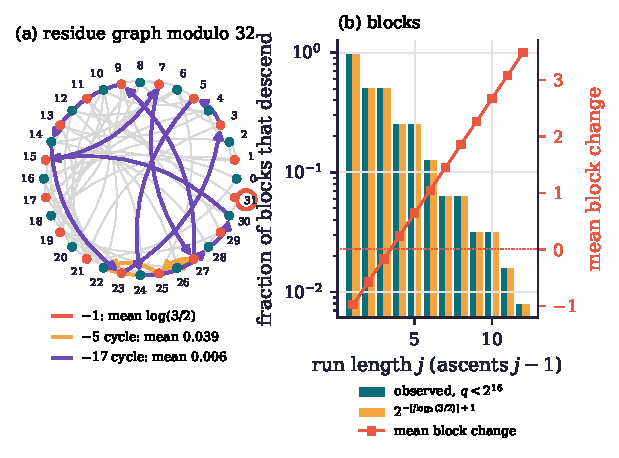
\includegraphics[width=\textwidth]{figures/ch5c_residue_blocks.pdf}
\caption{(a) The residue graph $G_5$ modulo $32$, its odd and even residues in two shades and its edges in grey, and three of its $91$ simple cycles of positive weight, the images of the cycles of $T$ on the negative integers, highlighted with their mean weights. (b) Blocks: the fraction of blocks of run length $j$ that descend, from an exact scan over $q<2^{16}$ and from the formula $2^{-\lceil j\log_2(3/2)\rceil+1}$ of \cref{prop:ch5c:block}, with the mean block change $(j-1)\log(3/2)+\log3-3\log2$ under the model.}
\label{fig:ch5c:residue}
\end{figure}

\section{What a pointwise potential must read}\label{sec:ch5c:surplus}

Residues modulo $2^d$ read $d$ bits of $x$. The chains of
\cref{prop:ch4:chain} show that the number of bits a potential must read is
unbounded, and the following proposition makes the requirement quantitative.

\begin{proposition}[Surplus along chains]\label{prop:ch5c:surplus}
Suppose $V(x)=\log x+\varphi(x)$ satisfies $V(S(x))<V(x)$ for every odd $x\ge3$.
Then for every $j\ge2$ and odd $q\ge1$,
\[
  \varphi(2^jq-1)-\varphi(2\cdot3^{j-1}q-1)\;>\;(j-1)\log\frac32 .
\]
In particular $\varphi$ is unbounded above or below, and
$\sup\varphi-\inf\varphi\ge(j-1)\log(3/2)$ for every $j$.
\end{proposition}

\begin{proof}
By \cref{prop:ch4:chain} the first $j-1$ strides from $x=2^jq-1$ are
$x_i=3^i2^{j-i}q-1$, each with $k=1$, and
$\log(x_{i+1}/x_i)=\log\bigl((3\cdot2^{j-i-1}q\cdot3^i-1)/(3^i2^{j-i}q-1)\bigr)
>\log(3/2)$, since $2(3^{i+1}2^{j-i-1}q-1)>3(3^i2^{j-i}q-1)$. Summing the
strict decreases $V(x_{i+1})<V(x_i)$ over $i=0,\dots,j-2$ gives
$\varphi(x_{j-1})-\varphi(x_0)<-\sum_i\log(x_{i+1}/x_i)<-(j-1)\log(3/2)$.
\end{proof}

So a pointwise potential must give the integer $2^jq-1$, whose binary expansion
ends in $j$ ones, a surplus of at least $(j-1)\log(3/2)$ over the integer
$2\cdot3^{j-1}q-1$ it becomes after its run of ascents. The surplus has to grow
without bound with the number of trailing ones, and trailing ones are the
simplest unbounded feature of the binary expansion. A potential that reads only
boundedly many bits cannot do this, which is \cref{thm:ch5c:residue} again; a
potential that reads the run length can, and the next section shows what
happens when it does.

\section{Block majorization}\label{sec:ch5c:block}

Let $x=2^jq-1$ with $q$ odd and $j\ge1$, so that $j-1=\vt(x+1)-1$ is the number
of ascending strides that follow. Majorize not over one stride but over the
whole \emph{block}: the $j-1$ ascents and the descent that ends them.

\begin{proposition}[Block map]\label{prop:ch5c:block}
For $x=2^jq-1$ with $q$ odd,
\begin{equation}\label{eq:ch5c:block}
  S^{(j)}(x)=\frac{3^jq-1}{2^{v}},\qquad v=\vt(3^jq-1)\ge1,
\end{equation}
and the block descends, $S^{(j)}(x)<x$, if and only if $v>j\log_2(3/2)$ (for
$x\ge3$). Under the model in which $q$ is uniform on odd residues, $v$ is
Geometric$(\tfrac12)$, the fraction of blocks of run length $j$ that descend is
$2^{-\lceil j\log_2(3/2)\rceil+1}$, and the mean change of $\log x$ over the block
is $(j-1)\log(3/2)+\log3-3\log2+O(1/x)$, which is negative for $j\le3$ and
positive for $j\ge4$.
\end{proposition}

\begin{proof}
By \cref{prop:ch4:chain}, $S^{(j-1)}(x)=2\cdot3^{j-1}q-1$, which is $\equiv1
\pmod4$; the next stride is $(3(2\cdot3^{j-1}q-1)+1)/2^k=(2\cdot3^jq-2)/2^k=
(3^jq-1)/2^{k-1}$ with $k-1=\vt(3^jq-1)$.
Comparing with $x=2^jq-1$, write $3^jq-1=2^vu$ with $u=S^{(j)}(x)$ odd; then $q(2^{j+v}-3^j)=2^v(2^jq-u)-1$, and $2^jq-u$ is odd.
If $2^{j+v}<3^j$ the left side is negative, so $u>2^jq>x$ and the block ascends.
If $2^{j+v}>3^j$ the left side is positive, so $2^jq-u$ is a positive odd integer, and $S^{(j)}(x)<x$ unless $2^jq-u=1$, that is, unless $S^{(j)}(x)=x$ and $x$ lies on a cycle consisting of a single block.
By the theorem of Steiner\index{Steiner, R. P.}~\cite{steiner1977} (see also \cite[Theorem~J]{lagarias1985}) the only such cycle is the trivial one, so for $x\ge3$ the block descends exactly when $2^{j+v}>3^j$, that is, when $v>j\log_2(3/2)$; the exact scan in \texttt{ch5c\_mm.py} agrees for every $q<2^{16}$ and $j\le12$.
For uniform odd $q$, $3^jq-1$ is uniform over
even residues, so $\Prob(v\ge i)=2^{-(i-1)}$. The threshold is the least
integer $v$ with $v>j\log_2(3/2)$, namely $\lceil j\log_2(3/2)\rceil$ when that
is not an integer, which it never is for $j\ge1$ since $\log_2(3/2)$ is
irrational; this gives the fraction. The mean change is $(j-1)\log(3/2)$ from
the ascents plus $\log3-\E[k]\log2$ with $\E[k]=\E[v]+1=3$ from the descent.
\end{proof}

The block is the natural MM unit: it is the shortest horizon over which the
surrogate can be made exact, since within a run of ascents the halving exponents
are forced to be $1$ and the only random quantity is the valuation $v$ at the
end. \Cref{fig:ch5c:residue}(b) shows the descent fractions, which the scan
reproduces exactly for $j\ge2$ (at $j=1$ it gives $1-2^{-15}$, because it includes the fixed point $x=1$), and the mean block change, which crosses zero between
$j=3$ and $j=4$. Blocks of run length four or more, that is, with three or more ascents, are, on average, net ascents.
Their rarity, $2^{-j}$ for run length $j$, is what makes the overall drift\index{drift}
negative: averaging over $j$ gives $\sum_j2^{-j}((j-1)\log(3/2)+\log3-3\log2)
=2\log(3/4)$, two strides' worth of the Syracuse drift, as it must.

\paragraph{Block potentials.} The block suggests the potential
$V_c(x)=\log x+c\,\vt(x+1)$, which pays in advance for the coming ascents.

\begin{proposition}[Run length potential]\label{prop:ch5c:runpot}
Let $V_c(x)=\log x+c\,\vt(x+1)$ with $c>\log(3/2)$. Then $V_c$ decreases at every
ascending stride from $x>1/(2(e^c-3/2))$, hence at every ascending stride when $c>\log(5/3)$ and at all but finitely many when $c\le\log(5/3)$.
The descending strides at which it fails to decrease are exactly those $x\mapsto y$, with $k$ halvings, that land on a $y$ with
$\vt(y+1)-1\ge(k\log2-\log3-\varepsilon(x))/c$. Under the model the fraction of
odd $x$ at which $V_c$ fails is
\[
  p(c)=\sum_{k\ge2}2^{-k}\,2^{-\lceil(k\log2-\log3)/c\rceil},
\]
which is $0.2087$ at $c=1$ and decreases to $0.1431$ as $c\downarrow\log(3/2)$,
and $V_c$ fails at a positive fraction of odd integers for every $c$.
\end{proposition}

\begin{proof}
At an ascending stride from $x$ with $\vt(x+1)=j\ge2$, by \eqref{eq:ch4:chain}
$\vt(S(x)+1)=j-1$ and $S(x)=(3x+1)/2$, so $V_c$ changes by $\log(3/2+1/(2x))-c$, which is negative exactly when $x>1/(2(e^c-3/2))$.
Ascending strides start at $x\ge3$, so this covers all of them when $c>\log(5/3)$; for $c\le\log(5/3)$ the stride $3\mapsto5$ fails, and for $c\le\log(11/7)$ also $7\mapsto11$ (the scan in \texttt{ch5c\_mm.py} lists the ascending failures).
At a descending stride with $k\ge2$ halvings, $\vt(x+1)=1$ and the
change is $\log3-k\log2+\varepsilon(x)+c(\vt(y+1)-1)$, which gives the stated
criterion. Under the model $k$ is Geometric$(\tfrac12)$, the descending strides being those with $k\ge2$, and $\vt(y+1)$ is an independent Geometric$(\tfrac12)$, so that $\Prob(\vt(y+1)-1\ge t)=2^{-t}$, and summing over $k$ gives $p(c)$;
the scan over odd $x<2^{20}$ gives $0.2087$ at $c=1$, matching the model to four
digits (\cref{fig:ch5c:runpot}). Positivity of $p(c)$ is clear from the $k=2$
term.
The integers fail at a positive fraction as well: if $x\equiv9\pmod{16}$ then $k=2$, $\vt(x+1)=1$ and $y=(3x+1)/4\equiv3\pmod4$, so $\vt(y+1)\ge2$ and $V_c$ changes by more than $\log(3/4)+c=c-\log(4/3)>0$, and these $x$ are one eighth of the odd integers. (For $c\le\log(3/2)$ the ascending strides, half of the odd integers, fail instead, by the first step of the proof.)
\end{proof}

\begin{figure}[ht]
\centering
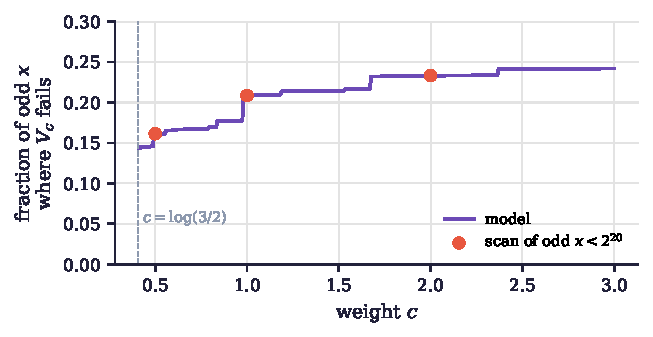
\includegraphics[width=\textwidth]{figures/ch5c_runpotential.pdf}
\caption{The fraction of odd integers at which the run length potential
$V_c=\log x+c\,\vt(x+1)$ fails to decrease over one stride, as a function of the
weight $c$: the model formula of \cref{prop:ch5c:runpot} and an exact scan of
odd $x<2^{20}$. The infimum, $0.143$, is approached as $c$ decreases to
$\log(3/2)$; below that value the ascending strides fail instead.}
\label{fig:ch5c:runpot}
\end{figure}

The run length potential does precisely what \cref{prop:ch5c:surplus} demands,
and it moves the obstruction rather than removing it. For $c>\log(5/3)$ it succeeds on every
ascent, and fails on the descents that land on an integer whose next run of
ascents is long enough to outweigh the halvings just gained. One can pay for
that run too, with a potential that reads the run after the next descent, and
then the failures move to the landing after that; the regress ends only with the
potential that reads the whole orbit to the first descent below $x$, which is
the stopping time\index{stopping time}, and whose finiteness is the conjecture. This is the
sense in which the MM approach locates the problem: each potential in this regress is
a truncation of the stopping time at some depth of the binary expansion, and
the conjecture asks, in effect, that the stopping time they truncate be finite.

\section{Majorization in expectation}\label{sec:ch5c:expectation}

There is one setting in which the majorization\index{MM algorithm} works perfectly. Under the stride model of
\cref{def:ch3:models}, take expectations in \eqref{eq:ch5c:stride}: with $k$
Geometric$(\tfrac12)$ the surrogate decrease has mean
$2\log2-\log3-1/(3x)$, which is $|\log(3/4)|$ up to $O(1/x)$, so $\log x$ is a strict supermartingale\index{martingale}\index{supermartingale} and
\cref{prop:absorb} gives absorption. Majorization in expectation is exactly the
supermartingale method, and it proves the model's version of the conjecture in
three lines. The pathwise version fails at the half of all odd integers where
$k=1$, and the preceding sections show that no repair by residues, by run
lengths, or by any bounded depth of the expansion restores it. The difference
between majorization\index{majorization} in expectation and pathwise majorization is the difference
between the model and the map, and it is the whole of the divergence half.

\section{What the approach offers}\label{sec:ch5c:verdict}

We can now state exactly what majorization\index{majorization} offers the Collatz problem.

For the cycle half it offers a reformulation: the cycle inequality is the
bound of the multiplicative majorizer summed around the cycle, the
window lemma\index{window lemma} is its minorizer, and the cycle half is the question of the
tightness of that majorizer along closed orbits. This is a clean statement and
nothing more; the arithmetic that would close the window is not supplied by
majorization.

For the divergence half it offers three impossibility results, each with a
proof: no residue potential (\cref{thm:ch5c:residue}), because the negative
cycles of $T$ are positive cycles of every residue graph; no potential $\log x+\varphi(x)$ with bounded $\varphi$
at all (\cref{prop:ch5c:surplus}); and no block potential of any weight
(\cref{prop:ch5c:runpot}). And it offers one structural fact: the block
decomposition is exact, each block's fate is
decided by the single valuation $\vt(3^jq-1)$, and under the model the blocks
form a renewal\index{renewal theory} process; the conjecture in descent
form is the statement that the sequence of blocks, started at any $n$,
reaches a block whose descent takes the orbit below $n$.

The conclusion is that majorization, pressed as hard as we are able to
press it, converts the conjecture into an equivalent termination statement with
an explicit and simple structure, and proves that the truncations of that
statement examined here, to boundedly many bits of $x$ or to a single run of
ascents, are false. What it does not do is produce the
unbounded depth argument. We believe that this is the right place to be stuck,
because, as \cref{chap:computation} will show, it is also where the automated termination provers and the $2$ adic analysis of \cref{prop:ch10b:residue}
are stuck, and three independent routes ending at the same wall is some
evidence that the wall is real.

\section*{Notes}

The negative cycle criterion for the existence of potentials is the
Bellman\index{Bellman, R.}~\cite{bellman1958} and Ford\index{Ford, L. R.}~\cite{ford1956} condition of shortest path theory, and the maximum cycle mean
is computed by Karp's algorithm\index{Karp, R. M.}~\cite{karp1978}; both are in any text on combinatorial
optimization. The observation that the negative integer cycles obstruct residue
based certificates\index{certificate} is, in the language of $2$ adic integers, the statement that $-1$, $-5$ and $-17$ lie in the exceptional set $E$ of \cref{chap:computation} (\cref{prop:ch10b:residue}); the cycles themselves are classical, see Lagarias\index{Lagarias, J. C.}~\cite{lagarias1985}.
Its formulation as a positive cycle in the residue graph, the surplus proposition and the run length potential are ours.
The block map
itself is the classical identity behind \cref{prop:ch4:chain} followed by one
descending stride; Hercher\index{Hercher, C.}~\cite[Lemma~8]{hercher2023} cites
Terras\index{Terras, R.}~\cite{terras1976} for the identity.
A cycle consisting of a single block is called a circuit, and Steiner\index{Steiner, R. P.}~\cite{steiner1977} showed that the trivial cycle is the only circuit~\cite[Theorem~J]{lagarias1985}; by the identity in the proof of \cref{prop:ch5c:block}, this is exactly the ``if'' half of the descent criterion for blocks, whose ``only if'' half is elementary.

\section*{Exercises}

\begin{exercise}
Verify by hand that the $-5$ cycle of $T$ maps to a closed walk of weight
$2\log3-3\log2$ in $G_d$ for every $d\ge2$, and locate its three residues in
$G_5$ in \cref{fig:ch5c:residue}(a).
\end{exercise}

\begin{exercise}
Show that the maximum cycle mean of $G_d$ would drop below $\log(3/2)$ if the
loop at $-1$ were deleted, compute the new maximum for $d=5$, and explain why
deleting it is not legitimate.
\end{exercise}

\begin{exercise}
Every odd $x\ge3$ is uniquely $2^jq-1$ with $q$ odd, and the block map sends it
to $S^{(j)}(x)=(3^jq-1)/2^v$. Show that under the model in which the residue of
$q$ is uniform, the pair $(j',v')$ of the next block is independent of the
current pair, with $j'$ and $v'$ independent Geometric$(\tfrac12)$, so that,
under the model, the sequence of blocks is a renewal\index{renewal theory} process. Compute the mean
number of strides per block and recover the Syracuse drift\index{drift}.
\end{exercise}

\begin{exercise}
Compute $p(c)$ of \cref{prop:ch5c:runpot} for $c=2$ and compare with the scan
value $0.2333$. Why does the failure fraction increase with $c$ for large $c$?
\end{exercise}

\begin{exercise}
Define the depth two potential $V^{(2)}_c(x)=\log x+c\,\vt(x+1)+c\,\vt(y+1)$,
where $y$ is the first element of the orbit after the next descent. Show that
it decreases at every stride except descents whose second landing has a long
run, and compute the model fraction of failures. Describe the general depth $h$
potential and its failure set.
\end{exercise}
